\documentclass[compress,blue]{beamer}
\logo{\includegraphics[width=0.12\textwidth]{stout_logo}\hspace{-2pt}}
% \usetheme{default}
%\usetheme{Boadilla}
%\usetheme{Bergen}
\usetheme{Berkeley}
%\usetheme{Goettingen}
%\usetheme{Hannover}
%\usetheme{Luebeck}
% \usetheme{Madrid}
%\usetheme{Montpellier}
%\usetheme{Rochester}
%\usetheme{Warsaw}

% \mode<presentation>
\usepackage{amsmath} \usepackage{graphicx}
\usepackage{amsfonts} \usepackage{amssymb}

\def\QED{{\ \vbox{\hrule\hbox{\vrule height1.3ex\hskip0.8ex\vrule}\hrule}}\par}
\def\ds{\displaystyle}
\newcommand{\pdiff}[2]{\frac{\partial #1}{\partial #2}}
\newcommand{\pdiffsec}[2]{\frac{\partial^2 #1}{\partial^2 #2}}
\newcommand{\diff}[2]{\frac{d #1}{d #2}}

%%%%%%%%%%%%%%% EITHER DEVELOP A CATCHY TITLE OR USE THE INDUSTRY SPONSOR NAME %%%%%%%%%%%%%%%
\title{The District Company}
%%%%%%%%%%%%%%% IF THE COMPANY NAME DOES NOT APPEAR, PLACE IT AFTER THE LIASON'S NAME %%%%%%%%%%%%%%%
%%%%%%%%%%%%%%% E.G. Steve Jobs, Apple Inc. %%%%%%%%%%%%%%%
\subtitle{Industry Liason: Dustin Jepperson}

%%%%%%%%%%%%%%% ENTER YOUR GROUP MEMBERS HERE %%%%%%%%%%%%%%%
\author{Megan Mortensen, Connor Phu, \\
Brian Dassow, Bella Nordahl}

%%%%%%%%%%%%%%% REPLACE THE BLUE DEVILS LOGO WITH THE COMPANY LOGO IF ONE EXISTS %%%%%%%%%%%%%%%
\titlegraphic{\includegraphics[width=0.33\textwidth]{pic_math_logo}\hspace{0cm}
\includegraphics[width=0.33\textwidth]{DistrictCompanylogo}}

\institute{\textbf{University of Wisconsin Stout} \\
}
\date{March 30, 2016}

\begin{document}

% this prints title, author etc. info from above
\frame{\titlepage}

%\frame{\frametitle{Outline}\tableofcontents[pausesections]}

%%%%%%%%%%%%%%% BELOW IS YOUR SLIDE DECK %%%%%%%%%%%%%%%
%%%%%%%%%%%%%%% CHANGE SLIDE TITLES, ETC. AS YOU DEEM APPROPRIATE %%%%%%%%%%%%%%%
%%%%%%%%%%%%%%%%%%%%%%%%%%%%%%%%%%%%%%%%%%%%%%%%%%%%%%%%%%%
%%%%%%%%%%%%%%% MUST INCLUDE:
%%%%%%%%%%%%%%% (1) Give a statement of the problem and tell why the problem is important
%%%%%%%%%%%%%%% (2) Brief statement of your results
%%%%%%%%%%%%%%% (3) Details about your approach to the problem  
%%%%%%%%%%%%%%% (4) More detailed presentation of your results
%%%%%%%%%%%%%%% (5) Restatement of the problem and the results
%%%%%%%%%%%%%%% (6) Suggested future work
%%%%%%%%%%%%%%% (7) Acknowledgements slide (Leave this slide in the deck, just edit accordingly.)
%%%%%%%%%%%%%%% %%%%%%%%%%%%%%% %%%%%%%%%%%%%%% %%%%%%%%%%%%%%%

\section{Introducing the Problem}

\begin{frame}{Problem Statement}
\setbeamertemplate{itemize items}[circle]
\begin{itemize}
	\item Interpret data to help the company make important business decisions
	\item Look at the correlation between events and concession sales
	\item Create and evaluate surveys to determine what customers want and need
\end{itemize}
\end{frame}


\section{Status Update}

\begin{frame}{Status Update}
\setbeamertemplate{itemize items}[circle]
\begin{itemize}
  \item New data overlap
  \item Class to organize and access data
  \item Use regression and heat maps to look at correlations 
\end{itemize}
\end{frame}


\section{Data Analysis}

\begin{frame}{Data Comparison}
\setbeamertemplate{itemize items}[circle]
\begin{rows}
\row{\textwidth}
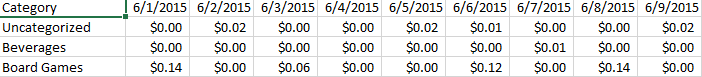
\includegraphics[width=10cm,height=2.5cm]{OriginalData}
\row{\textwidth}
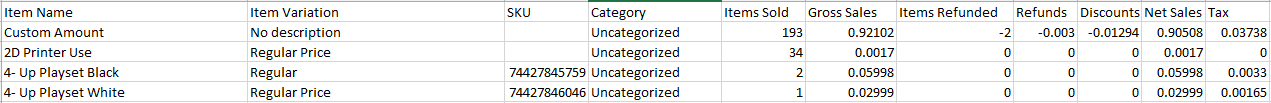
\includegraphics[width=10cm,height=2.5cm]{NewData}
\end{rows}
\end{frame}

\begin{frame}{New Data}
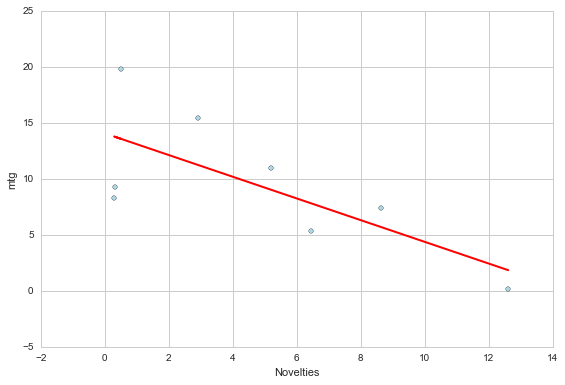
\includegraphics[width=7cm,height=6cm]{mtg_novelties}
\end{frame}

\begin{frame}{Class}
\setbeamertemplate{itemize items}[circle]
\begin{itemize}
	\item Organizes our new data
	\item Sums up values for taxes, net sales, gross sales, etc
\end{itemize}
\end{frame}

\begin{frame}{Regression}
\begin{columns}
\hspace{-5cm}
\column{}
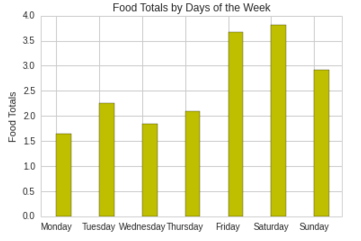
\includegraphics[width=5cm,height=4cm]{FoodTotals}
\column{}
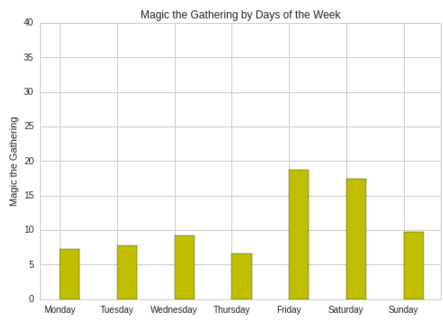
\includegraphics[width=5cm,height=4cm]{MTG}
\end{columns}
\end{frame}

\begin{frame}{Regression}
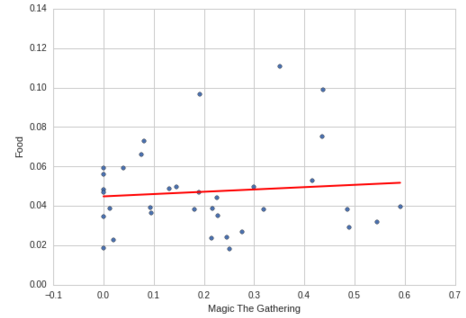
\includegraphics[width=7cm,height=6cm]{MTGandFoodRegression}
\end{frame}

\begin{frame}{Heat Maps}
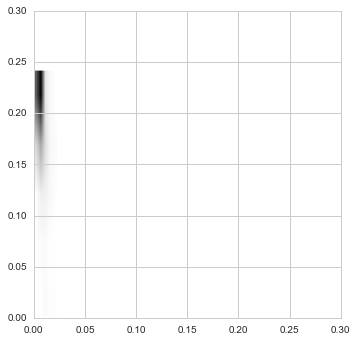
\includegraphics[width=7cm,height=6cm]{FoodandCandy}
\end{frame}

\begin{frame}{Heat Maps}
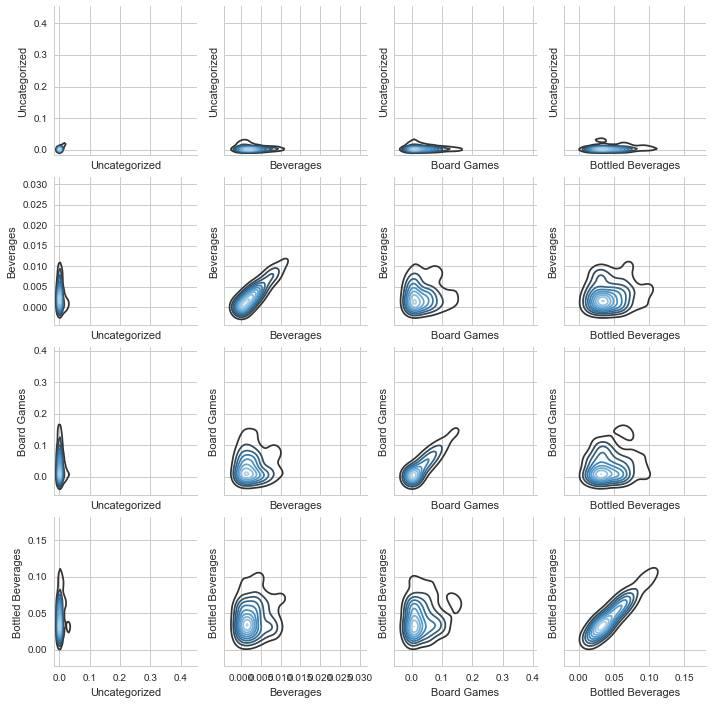
\includegraphics[width=7cm,height=6cm]{Cool}
\end{frame}



\end{document} 
